% vim: set tw=78 aw sw=2 sts=2 noet:
\documentclass{beamer}

\usepackage[english]{babel}
\usepackage{comment}
\usepackage{array}
\usepackage{listings}

\setbeamertemplate{navigation symbols}{}
\setbeamertemplate{footline}[frame number]
\setbeamertemplate{caption}{Source: \insertcaption}

\AtBeginSection[]{
  \begin{frame}
	\vfill
	\centering
	\begin{beamercolorbox}[center]{title}
	  \usebeamerfont{title}\insertsectionhead\par
	\end{beamercolorbox}
	\vfill
  \end{frame}
}

\mode<presentation>

\title{Leveraging the power of C++ for efficient machine learning on embedded
devices}
\subtitle{}
\author{Adrian Stanciu\\{\small adrian.stanciu.pub@gmail.com}}
\date{}
\institute{NDC TechTown, 2023}

\begin{document}

\frame{\titlepage}

\begin{frame}{About me}
  \begin{itemize}
	\item I am a software engineer from Romania
	\item I have a bachelor's degree in computer science from Politehnica
	University of Bucharest
	\item I have a master's degree in computer and network security from
	Politehnica University of Bucharest
	\item I have 12 years of professional experience in Linux system
	programming
	\item My main programming languages are C and C++
	\item I am interested in algorithms, data structures and operating systems
	\item I work at Bitdefender, where I develop security software solutions
	for routers
  \end{itemize}
\end{frame}

\begin{frame}{Disclaimer}
  \begin{itemize}
	\item This presentation is based on a personal project I worked on in my
	spare time and it is not directly related to the work I do at Bitdefender
	\item The outcome of this project is just a proof of concept
	\item All mistakes are mine
  \end{itemize}
\end{frame}

\begin{frame}{Agenda}
  \begin{itemize}
	\item Motivation
	\item Image classification
	\item Hand gesture recognition
	\item Best practices
	\item Summary
  \end{itemize}
\end{frame}

% vim: set tw=78 aw sw=2 sts=2 noet:

\section{Motivation}

\begin{frame}{Machine Learning (ML)}
  \begin{itemize}
	\item Subfield of Artificial Inteligence (AI)
	\item Enables computers to learn from data and then use that knowledge to
	make predictions
	\item Applications:
	  \begin{itemize}
		\item Computer vision
		\item Medicine
		\item Search engines
	  \end{itemize}
  \end{itemize}
\end{frame}

\begin{frame}{Embedded devices}
  \begin{itemize}
	\item Computing devices designed to perform specific tasks within larger systems
	\item Applications:
	  \begin{itemize}
		\item Consumer electronics (mobile phones, smart TVs)
		\item Home automation (thermostats, lighting control systems)
		\item Medical equipment (pacemakers, insulin pumps)
	  \end{itemize}
	\item Characteristics:
	  \begin{itemize}
		\item Limited hardware resources
		\item Low power consumption
		\item May have real-time performance constraints
	  \end{itemize}
  \end{itemize}
\end{frame}

\begin{frame}{Machine learning on embedded devices}
  \begin{itemize}
	\item Alternative to cloud-based machine learning
	\item Advantages:
	  \begin{itemize}
		\item Real-time processing
		\item Low latency
		\item Reduced bandwidth usage
		\item Offline operation
		\item Improved privacy
	  \end{itemize}
	\item Disadvantages:
	  \begin{itemize}
		\item Compatibility with various hardware and software platforms
		\item Slower updates
	  \end{itemize}
  \end{itemize}
\end{frame}

\begin{frame}{Using C++ for machine learning on embedded devices}
C++ is widely used in embedded systems:
  \begin{itemize}
	\item Was designed with efficiency in mind
	\item Provides both low-level access to hardware resources and high-level
	abstractions
	\item Is supported on most hardware and software platforms
  \end{itemize}
\end{frame}


% vim: set tw=78 aw sw=2 sts=2 noet:

\section{Image classification}

\begin{frame}{Supervised learning}
Machine learning paradigm in which an algorithm learns from labeled training
data to make predictions or decisions
  \begin{figure}
	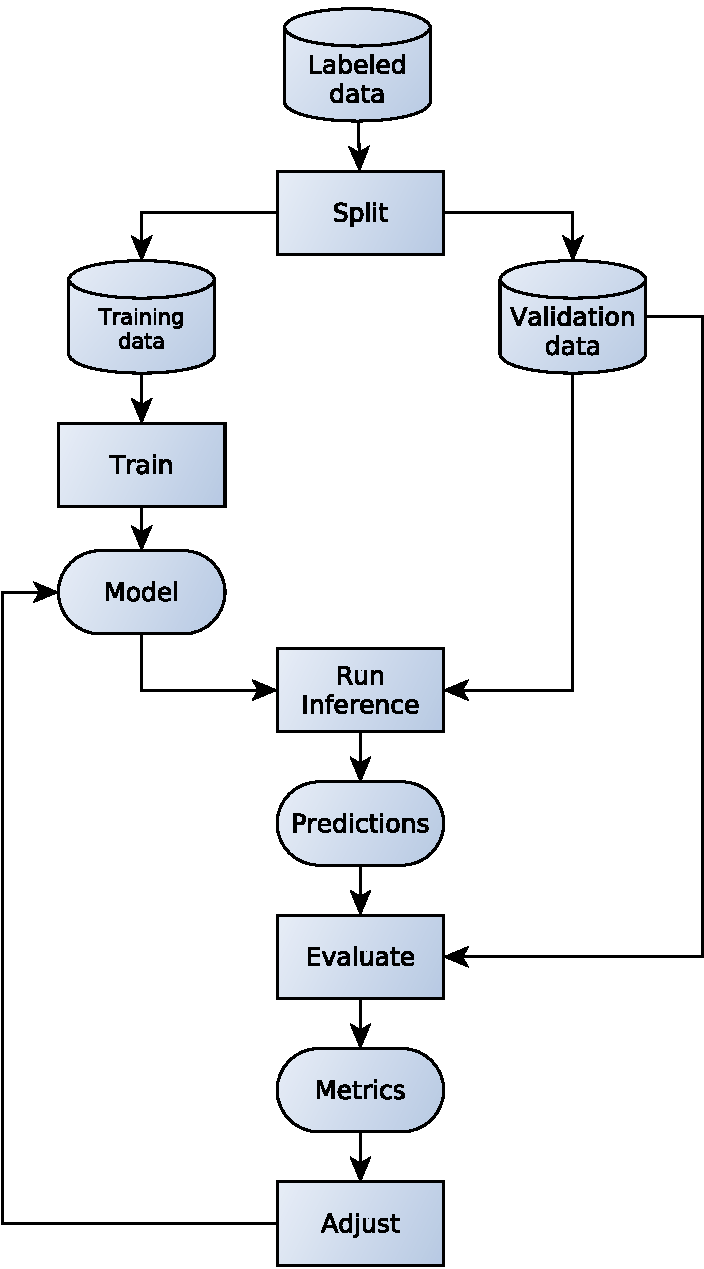
\includegraphics[width=\linewidth,height=0.75\textheight,keepaspectratio]{images/supervised_learning.pdf}
  \end{figure}
\end{frame}

\begin{frame}{Supervised learning}
  \begin{figure}
	
\includegraphics[width=\linewidth,height=0.75\textheight,keepaspectratio]{images/xkcd_machine_learning.png}
	\caption{xkcd.com}
  \end{figure}
\end{frame}

\begin{frame}{Neural network (NN)}
  \begin{figure}
	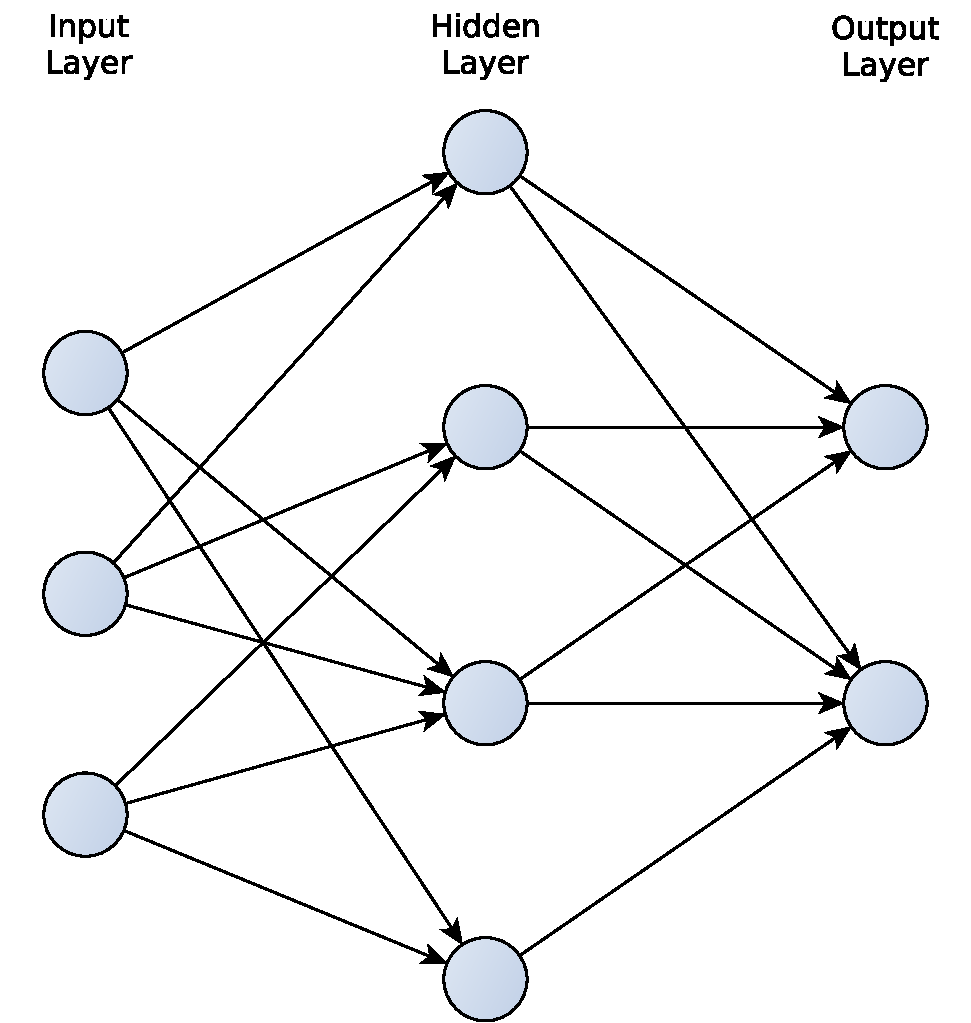
\includegraphics[width=\linewidth,height=0.75\textheight,keepaspectratio]{images/neural_network.pdf}
  \end{figure}
\end{frame}

\begin{frame}{Neural network (NN)}
  \begin{figure}
	
\includegraphics[width=\linewidth,height=\textheight,keepaspectratio]{images/monkeyuser_ai_care.png}
	\caption{monkeyuser.com}
  \end{figure}
\end{frame}

\begin{frame}{Convolutional neural network (CNN)}
  \begin{itemize}
	\item Efficient in image classification
	\item A convolutional layer can apply filters to detect:
	  \begin{itemize}
		\item Edges
		\item Shapes
		\item Objects
	  \end{itemize}
  \end{itemize}
\end{frame}

\begin{frame}{Hardware setup}
  \begin{itemize}
	\item Raspberry Pi 4 model B:
	  \begin{itemize}
		\item Quad core Cortex-A72 (ARM v8) 64-bit SoC @ 1.8GHz
		\item 4GB RAM
	  \end{itemize}
	\item 8GB microSD card
	\item Raspberry Pi Camera module 3
  \end{itemize}
  \begin{figure}
	\includegraphics[width=\linewidth,height=\textheight,keepaspectratio]{images/rpi.pdf}
  \end{figure}
\end{frame}

\begin{frame}{Software}
  \begin{itemize}
	\item 64-bit Raspberry Pi OS
	\item gcc with C++20 support
	\item TensorFlow Lite
	\item OpenCV
  \end{itemize}
\end{frame}

\begin{frame}{TensorFlow Lite}
  \begin{itemize}
	\item Optimized pre-trained models
	\item C++ and Python APIs
  \end{itemize}
\end{frame}

\begin{frame}{Data organization}
  \begin{itemize}
	\item A tensor is an array in which data (both input and output) is organized
	\item For 2D images the size of the tensor is computed as \\ \texttt{width * height *
	channels * sizeof(type)}
  \end{itemize}
\end{frame}

\begin{frame}{MobileNet pre-trained model}
  \begin{itemize}
	\item CNN architecture created by Google
	\item 1000 classes (labels)
	\item Labels are stored separate from the model:
	  \begin{itemize}
		\item \texttt{labels\_mobilenet\_quant\_v1\_224.txt} (11KB)
		\item \texttt{mobilenet\_v1\_1.0\_224\_quant.tflite} (4.1MB)
	  \end{itemize}
	\item Tensor dimensions:
	  \begin{itemize}
		\item 224x224 pixels images
		\item 3 color channels per pixel (RGB)
		\item Type is \texttt{uint8\_t}
	  \end{itemize}
  \end{itemize}
\end{frame}

\begin{frame}{Algorithm}
  \begin{enumerate}
	\item Load model and labels
	\item Build interpreter
	\item Allocate input and output tensors
	\item Read image
	\item Resize image
	\item Copy resized image to input tensor
	\item Run inference
	\item Extract results from output tensors
  \end{enumerate}
\bigskip
Steps 4-8 can be repeated multiple times
\end{frame}

\begin{frame}[fragile]{1. Load model and labels}
  \lstset{basicstyle=\ttfamily\small, numbers=left, columns=fullflexible}
  \begin{lstlisting}
// const char *model_path;
// const char *labels_path;

std::unique_ptr<tflite::FlatBufferModel> model{
  tflite::FlatBufferModel::BuildFromFile(model_path)
};

std::ifstream labels_ifs{labels_path};
std::string label;
std::vector<std::string> labels;
while (getline(labels_ifs, label)) {
  labels.push_back(std::move(label));
}

  \end{lstlisting}
\end{frame}

\begin{frame}[fragile]{2. Build interpreter}
  \lstset{basicstyle=\ttfamily\small, numbers=left, columns=fullflexible}
  \begin{lstlisting}
// std::unique_ptr<tflite::FlatBufferModel> model;
// int num_threads;

tflite::ops::builtin::BuiltinOpResolver resolver;
tflite::InterpreterBuilder builder{*model, resolver};

builder.SetNumThreads(num_threads);

std::unique_ptr<tflite::Interpreter> interpreter;
builder(&interpreter);
  \end{lstlisting}
\end{frame}

\begin{frame}[fragile]{3. Allocate input and output tensors}
  \lstset{basicstyle=\ttfamily\small, numbers=left, columns=fullflexible}
  \begin{lstlisting}
// std::unique_ptr<tflite::Interpreter> interpreter;

interpreter->AllocateTensors();
  \end{lstlisting}
\end{frame}

\begin{frame}[fragile]{4. Read image}
  \lstset{basicstyle=\ttfamily\small, numbers=left, columns=fullflexible}
  \begin{lstlisting}
// const char *image_path;

cv::Mat image{cv::imread(image_path)};
  \end{lstlisting}
\end{frame}

\begin{frame}[fragile]{5. Resize image}
  \lstset{basicstyle=\ttfamily\small, numbers=left, columns=fullflexible}
  \begin{lstlisting}
// cv::Mat image;
// int required_image_width;
// int required_image_height;

cv::Mat resized_image;
cv::resize(
  image,
  resized_image,
  cv::Size{required_image_width, required_image_height}
);
  \end{lstlisting}
\end{frame}

\begin{frame}[fragile]{6. Copy resized image to uint8\_t-typed input tensor}
  \lstset{basicstyle=\ttfamily\small, numbers=left, columns=fullflexible}
  \begin{lstlisting}
// std::unique_ptr<tflite::Interpreter> interpreter;
// cv::Mat resized_image;

std::memcpy(
  interpreter->typed_input_tensor<uint8_t>(0),
  resized_image.data,
  resized_image.total() * resized_image.elemSize()
);
  \end{lstlisting}
\end{frame}

\begin{frame}[fragile]{6. Copy resized image to float-typed input tensor - Wrong!}
  \lstset{basicstyle=\ttfamily\small, numbers=left, columns=fullflexible}
  \begin{lstlisting}
// std::unique_ptr<tflite::Interpreter> interpreter;
// cv::Mat resized_image;

std::memcpy(
  interpreter->typed_input_tensor<float>(0),
  resized_image.data,
  resized_image.total() * resized_image.elemSize()
);
  \end{lstlisting}
\end{frame}

\begin{frame}[fragile]{6. Copy resized image to float-typed input tensor - Correct}
  \lstset{basicstyle=\ttfamily\small, numbers=left, columns=fullflexible}
  \begin{lstlisting}
// std::unique_ptr<tflite::Interpreter> interpreter;
// cv::Mat resized_image;

auto idx = 0;
for (auto row = 0; row < resized_image.rows; ++row) {
  for (auto col = 0; col < resized_image.cols; ++col) {
    auto pixel = resized_image.at<cv::Vec3b>(row, col);
    for (auto ch = 0; ch < pixel.channels; ++ch) {
      tensor_data[idx++] = pixel.val[ch];
    }
  }
}
  \end{lstlisting}
\end{frame}

\begin{frame}[fragile]{7. Run inference}
  \lstset{basicstyle=\ttfamily\small, numbers=left, columns=fullflexible}
  \begin{lstlisting}
// std::unique_ptr<tflite::Interpreter> interpreter;

interpreter->Invoke();
  \end{lstlisting}
\end{frame}

\begin{frame}[fragile]{8. Extract results from uint8\_t-typed output tensors}
  \lstset{basicstyle=\ttfamily\small, numbers=left, columns=fullflexible}
  \begin{lstlisting}
// std::unique_ptr<tflite::Interpreter> interpreter;
// std::vector<std::string> labels;

std::span<uint8_t> probabilities{
  interpreter->typed_output_tensor<uint8_t>(0),
  labels.size()
};
  \end{lstlisting}
\end{frame}

\begin{frame}[fragile]{8. Extract results from float-typed output tensors}
  \lstset{basicstyle=\ttfamily\small, numbers=left, columns=fullflexible}
  \begin{lstlisting}
// std::unique_ptr<tflite::Interpreter> interpreter;
// std::vector<std::string> labels;

std::span<float> probabilities{
  interpreter->typed_output_tensor<float>(0),
  labels.size()
};
  \end{lstlisting}
\end{frame}

\begin{frame}{Demo}
  \ttfamily \$ libcamera-jpeg --width=640 --height=480 -o out.jpeg
  \begin{figure}
	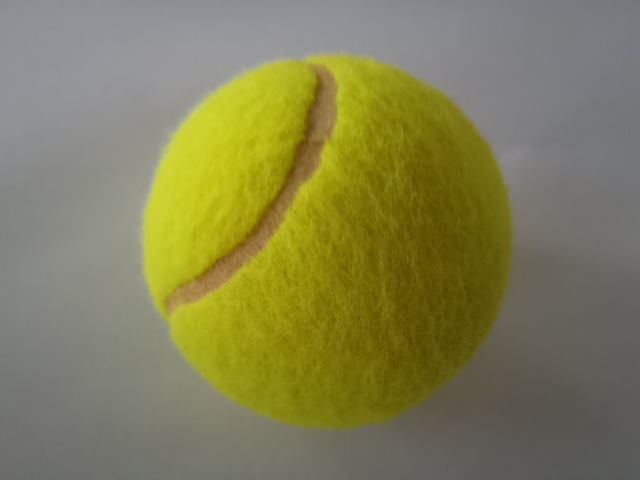
\includegraphics[width=0.5\linewidth,height=0.5\textheight,keepaspectratio]{../images/tennis_ball_input.jpeg}%
	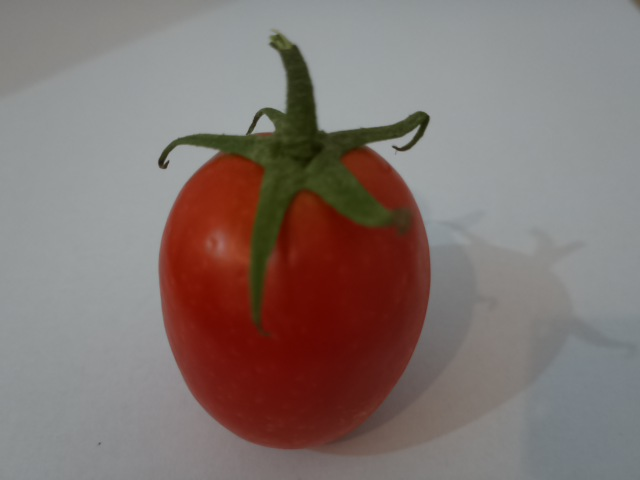
\includegraphics[width=0.5\linewidth,height=0.5\textheight,keepaspectratio]{images/tomato.jpeg}
  \end{figure}
\end{frame}

\begin{frame}{Demo - Good results}
  \begin{figure}
	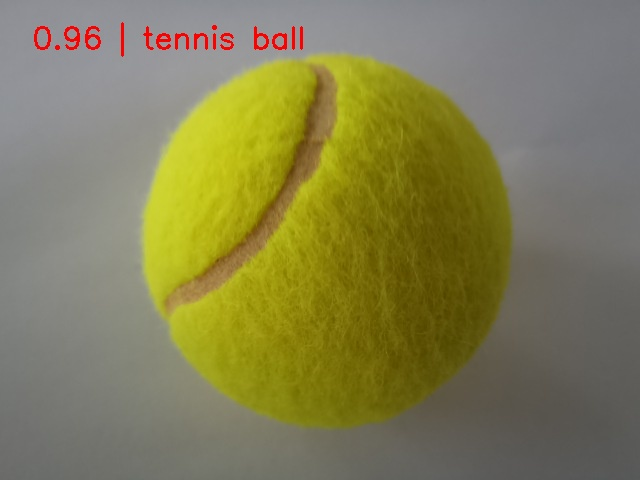
\includegraphics[width=\linewidth,height=0.5\textheight,keepaspectratio]{images/tennis_ball_output.jpeg}
  \end{figure}
  \ttfamily 0.96 | tennis ball
\end{frame}

\begin{frame}{Demo - Bad results}
  \begin{figure}
	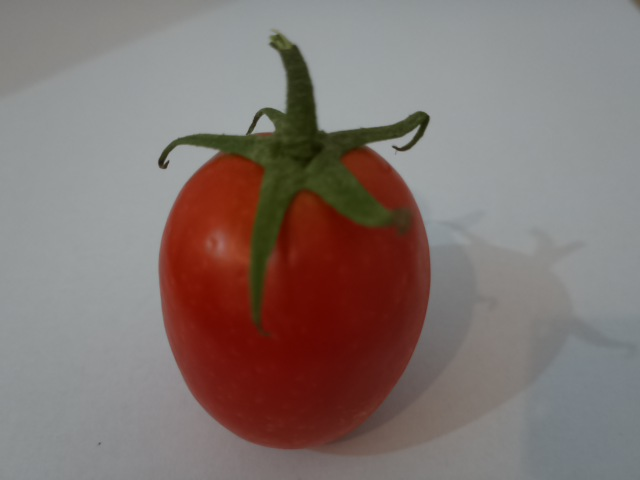
\includegraphics[width=\linewidth,height=0.5\textheight,keepaspectratio]{images/tomato.jpeg}
  \end{figure}
  \ttfamily 0.30 | vase \\
  \ttfamily 0.25 | bell pepper \\
  \ttfamily ambiguous results
\end{frame}

\begin{frame}{Demo - Bad results explanation}
  \ttfamily \$ grep "tomato" labels\_mobilenet\_quant\_v1\_224.txt \\
  \ttfamily \$
\end{frame}

\begin{frame}{Performance}
  \begin{itemize}
	\item Compilation duration: 35s
	\item Running duration: 1s
  \end{itemize}
  \begin{table}
    {\tiny
	\begin{tabular}{|c|c|}
	  \hline
		\textbf{Number of threads} & \textbf{Inference duration (ms)} \\
	  \hline
		1 & 102 \\
	  \hline
		2 & 56 \\
	  \hline
		3 & 41 \\
	  \hline
		4 & 33 \\
	  \hline
		5 & 110 \\
	  \hline
	\end{tabular}
	}
  \end{table}
  \begin{figure}
	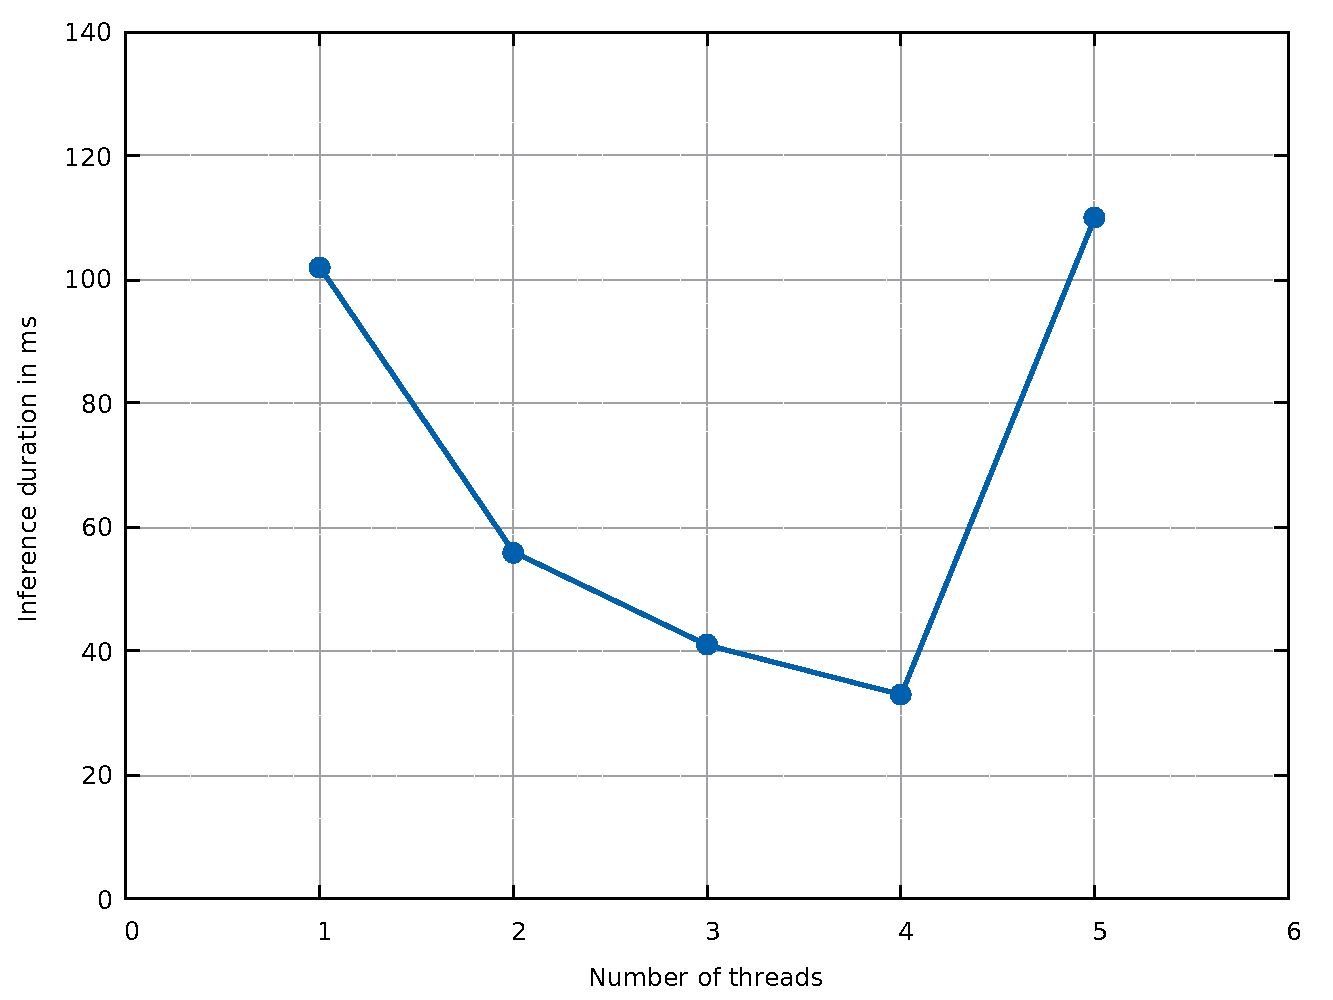
\includegraphics[width=\linewidth,height=0.5\textheight,keepaspectratio]{images/inference_duration.pdf}
  \end{figure}
  \begin{itemize}
	\item Memory consumption with 4 threads: 93MB
  \end{itemize}
\end{frame}

\begin{frame}{Comparision with Python}
Comparision made with TensorFlow Lite's \texttt{label\_image.py}
  \begin{table}
	\begin{tabular}{c|c|c|}
	  \cline{2-3}
		& \textbf{C++} & \textbf{Python} \\
	  \hline
		\multicolumn{1}{|c|}{\textbf{Running duration (s)}} & 1 & 7 \\
	  \hline
	\end{tabular}
  \end{table}
  \begin{table}
	\begin{tabular}{|c|c|c|}
	  \hline
		\textbf{Number of threads} & \multicolumn{2}{c|}{\textbf{Inference duration (ms)}} \\
	  \cline{2-3}
		& \hspace{0.35cm} \textbf{C++} \hspace{0.35cm} & \textbf{Python} \\
	  \hline
		1 & 102 & 118 \\
	  \hline
		2 & 56 & 62 \\
	  \hline
		3 & 41 & 42 \\
	  \hline
		4 & 33 & 33 \\
	  \hline
		5 & 110 & 170 \\
	  \hline
	\end{tabular}
  \end{table}
  \begin{table}
	\begin{tabular}{c|c|c|}
	  \cline{2-3}
		& \textbf{C++} & \textbf{Python} \\
	  \hline
		\multicolumn{1}{|c|}{\textbf{Memory consumption with 4 threads (MB)}} & 93 & 320 \\
	  \hline
	\end{tabular}
  \end{table}
\end{frame}


% vim: set tw=78 aw sw=2 sts=2 noet:

\section{Hand gesture recognition}

\begin{frame}{Rock-Paper-Scissors}
  \begin{figure}
	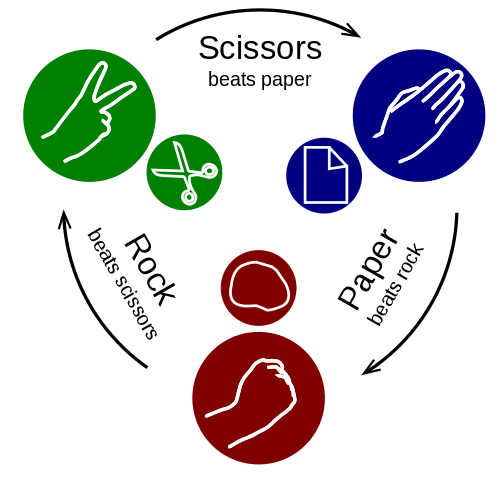
\includegraphics[width=\linewidth,height=0.75\textheight,keepaspectratio]{images/502px-Rock-paper-scissors.svg.png}
	\caption{wikipedia.org}
  \end{figure}
\end{frame}

\begin{frame}{Data}
  \begin{itemize}
	\item Google MediaPipe's Rock-Paper-Scissors dataset for hand gesture
	recognition
	  \begin{itemize}
		\item Contains 125 images for each class
		\item Images have various sizes
		\item Images have 3 color channels per pixel (RGB)
	  \end{itemize}
	\item Laurence Moroney's Rock-Paper-Scissors dataset (published by Sani
	Kamal on Kaggle)
	  \begin{itemize}
		\item Contains 964 images for each class split into training data
		(840) and testing data (124)
		\item Images are 300x300 pixels
		\item Images have 3 color channels per pixel (RGB)
	  \end{itemize}
  \end{itemize}
\end{frame}

\begin{frame}{Train a Rock-Paper-Scissors model}
  \begin{itemize}
	\item Transfer learning from a ResNet50 model
	\item 80/20 split between training and validation data
	\item Run in Python, on a laptop
  \end{itemize}
  \begin{table}
	\begin{tabular}{|c|c|c|}
	  \hline
		\textbf{Dataset} & \textbf{Train duration} & \textbf{Model size (MB)} \\
	  \hline
		Small & 2m15s & 23 \\
	  \hline
		Big & 7m10s & 23 \\
	  \hline
	\end{tabular}
  \end{table}
\end{frame}

\begin{frame}{Test the Rock-Paper-Scissors model}
  \begin{itemize}
	\item Using the testing data of the big dataset (124 images per class)
	\item Small dataset results:
  \begin{table}
	\begin{tabular}{|c|c|c|}
	  \hline
		\textbf{Gesture} & \textbf{Correct predictions} & \textbf{Accuracy (\%)} \\
	  \hline
		Rock & 108 & 87.09 \\
	  \hline
		Paper & 124 & 100 \\
	  \hline
		Scissors & 8 & 6.45 \\
	  \hline
	  \hline
		All & 240 out of 372 & 64.51 \\
	  \hline
	\end{tabular}
  \end{table}
	\item Big dataset results:
  \begin{table}
	\begin{tabular}{|c|c|c|}
	  \hline
		\textbf{Gesture} & \textbf{Correct predictions} & \textbf{Accuracy (\%)} \\
	  \hline
		Rock & 124 & 100 \\
	  \hline
		Paper & 122 & 98.38 \\
	  \hline
		Scissors & 97 & 78.22 \\
	  \hline
	  \hline
		All & 343 out of 372 & 92.20 \\
	  \hline
	\end{tabular}
  \end{table}
  \end{itemize}
\end{frame}

\begin{frame}{Performance}
  \begin{itemize}
	\item Compilation duration (on Raspberry Pi): 35s
	\item Binary size: 67KB
	\item Running duration: 1s
  \end{itemize}
  \begin{table}
    {\tiny
	\begin{tabular}{|c|c|}
	  \hline
		\textbf{Number of threads} & \textbf{Inference duration (ms)} \\
	  \hline
		1 & 151 \\
	  \hline
		2 & 98 \\
	  \hline
		3 & 80 \\
	  \hline
		4 & 71 \\
	  \hline
		5 & 189 \\
	  \hline
	\end{tabular}
	}
  \end{table}
  \begin{figure}
	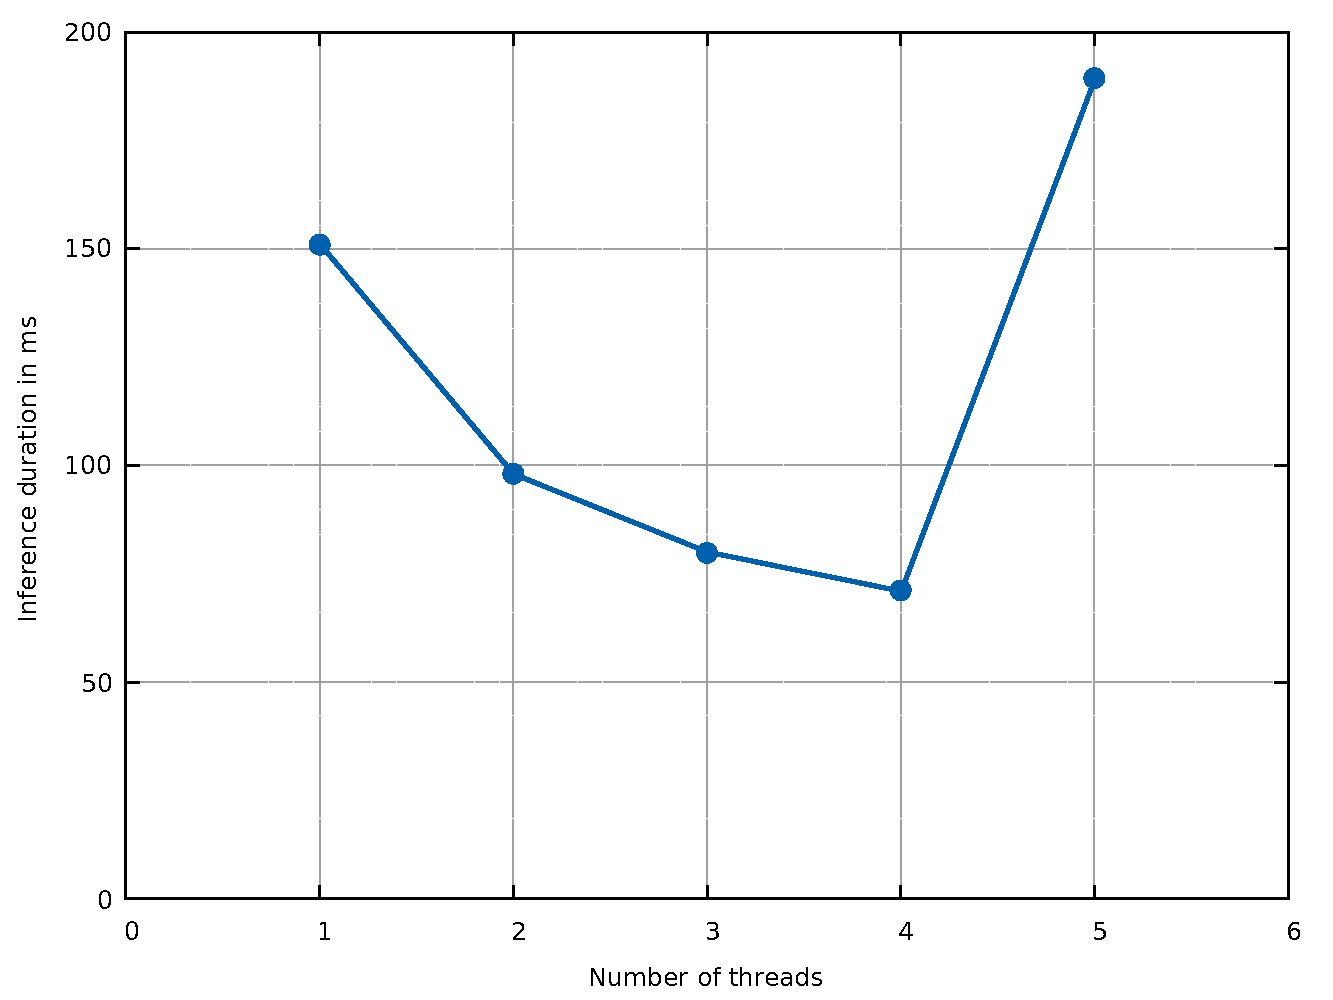
\includegraphics[width=\linewidth,height=0.45\textheight,keepaspectratio]{images/inference_duration_rps.pdf}
  \end{figure}
  \begin{itemize}
	\item Memory consumption with 4 threads: 118MB
  \end{itemize}
\end{frame}

\begin{frame}{Capture camera stream}
  \begin{itemize}
	\item libcamera backend
	\item gstreamer middleware
	\item OpenCV frontend
  \end{itemize}
\end{frame}

\begin{frame}[fragile]{Capture camera stream}
  \lstset{basicstyle=\ttfamily\small, showstringspaces=false, numbers=left,
  columns=fullflexible}
  \begin{lstlisting}
static constexpr const char *GstreamerPipeline{R"(
    libcamerasrc !
    video/x-raw,
    width=(int)640,
    height=(int)480,
    framerate=(fraction)10/1 !
    videoconvert !
    appsink
)"};

cv::VideoCapture camera{
  GstreamerPipeline,
  cv::CAP_GSTREAMER
};

cv::Mat image;
camera.read(image);
  \end{lstlisting}
\end{frame}

\begin{frame}{Live inference}
  \begin{enumerate}
	\item Create image classifier
	\item Open camera
	\item Do in a loop:
	\begin{enumerate}
	  \item Read image from camera
	  \item Use classifier to run inference on image
	  \item Show predictions
	\end{enumerate}
  \end{enumerate}
\end{frame}

\begin{frame}{Rock-Paper-Scissors game}
On each round the AI:
  \begin{enumerate}
	\item Chooses Rock, Paper or Scissors uniformly at random
	\item Infers the human's hand gesture
	\item Computes the outcome
  \end{enumerate}
\end{frame}


% vim: set tw=78 aw sw=2 sts=2 noet:

\section{Best practices}

\begin{frame}{Best practices}
  \begin{itemize}
	\item Integer quantization optimization
	\item Cross-compilation
	\item Binary size analysis
	\item Updates
  \end{itemize}
\end{frame}

\begin{frame}{Integer quantization optimization}
  \begin{itemize}
	\item The process of converting 32-bit floating-point numbers to the 8-bit integer numbers
	\item Reduces the size of the model and decreases inference duration at the expense of accuracy
  \end{itemize}
\end{frame}

\begin{frame}{Cross-compilation}
  \begin{itemize}
	\item The process to compile code for one system, named target (e.g.
	aarch64), on a different system, named host (e.g. x86\_64)
	\item Enables faster builds
  \end{itemize}
\end{frame}

\begin{frame}[fragile]{Binary size analysis}
Using Google's Bloaty McBloatface \\
\ttfamily \$ bloaty image\_classifier -d symbols
  \lstset{basicstyle=\tiny, numbers=left}
  \begin{lstlisting}
    FILE SIZE        VM SIZE
 --------------  --------------
  44.1%  29.5Ki  48.2%  29.5Ki    [section .text]
   8.3%  5.53Ki   9.0%  5.53Ki    [section .dynstr]
   7.7%  5.12Ki   8.4%  5.12Ki    [section .eh_frame]
   7.3%  4.90Ki   8.0%  4.90Ki    [section .rela.dyn]
   5.4%  3.59Ki   0.0%       0    [Unmapped]
   5.0%  3.38Ki   5.5%  3.38Ki    [section .dynsym]
   4.8%  3.18Ki   5.2%  3.18Ki    [section .rodata]
   2.9%  1.97Ki   3.2%  1.97Ki    [section .rela.plt]
   2.7%  1.81Ki   0.0%       0    [ELF Headers]
   2.0%  1.37Ki   2.2%  1.37Ki    [section .data.rel.ro]
   2.0%  1.34Ki   2.2%  1.34Ki    [section .plt]
   1.6%  1.07Ki   1.7%  1.07Ki    [section .eh_frame_hdr]
   1.1%     760   1.2%     760    [section .gcc_except_table]
   1.0%     696   1.1%     696    [section .got.plt]
   0.9%     624   1.0%     624    [section .dynamic]
   0.9%     598   1.0%     598    [LOAD #2 [RX]]
   0.8%     530   0.9%     579    [11 Others]
   0.4%     288   0.5%     288    [section .gnu.version]
   0.4%     274   0.0%       0    [section .shstrtab]
   0.4%     244   0.4%     244    [section .gnu.hash]
   0.3%     208   0.3%     208    [section .gnu.version_r]
 100.0%  66.9Ki 100.0%  61.3Ki    TOTAL
  \end{lstlisting}
\end{frame}

\begin{frame}[fragile]{Binary size analysis}
If compiled with debug info (\texttt{-g}) \\
\ttfamily \$ bloaty image\_classifier -d symbols
  \lstset{basicstyle=\tiny, numbers=left}
  \begin{lstlisting}
    FILE SIZE        VM SIZE    
 --------------  -------------- 
  42.0%  1.76Mi   0.0%       0    [section .debug_info]
  40.8%  1.71Mi   0.0%       0    [section .debug_str]
   8.8%   377Ki   0.0%       0    [section .debug_loc]
   3.4%   145Ki   0.0%       0    [section .debug_ranges]
   1.9%  82.6Ki   0.0%       0    [section .debug_line]
   1.3%  53.9Ki  53.1%  32.6Ki    [87 Others]
   0.5%  22.3Ki   0.0%       0    [section .debug_abbrev]
   0.1%  5.25Ki   7.5%  4.61Ki    std::__introsort_loop<>()
   0.1%  5.07Ki   0.0%       0    [section .strtab]
   0.1%  4.85Ki   0.0%       0    [section .symtab]
   0.1%  4.09Ki   6.7%  4.09Ki    [section .dynstr]
   0.1%  3.76Ki   5.1%  3.11Ki    std::__adjust_heap<>()
   0.1%  3.63Ki   4.8%  2.97Ki    std::__insertion_sort<>()
   0.1%  3.59Ki   0.0%       0    [Unmapped]
   0.1%  3.56Ki   3.6%  2.18Ki    cvflann::anyimpl::big_any_policy<>
   0.1%  3.34Ki   0.0%       0    [section .debug_aranges]
   0.1%  3.15Ki   3.4%  2.07Ki    cvflann::anyimpl::small_any_policy<>
   0.1%  3.06Ki   4.9%  2.99Ki    ic::ImageClassifier::run()
   0.1%  2.97Ki   2.0%  1.23Ki    cvflann::anyimpl::typed_base_any_policy<>
   0.1%  2.83Ki   4.4%  2.71Ki    ic::ImageClassifier::ImageClassifier()
   0.1%  2.78Ki   4.5%  2.75Ki    main
 100.0%  4.19Mi 100.0%  61.3Ki    TOTAL
  \end{lstlisting}
\end{frame}

\begin{frame}{Updates}
The model can be updated:
  \begin{itemize}
	\item Together with the application (use \texttt{\#embed} from C23 and
	replace \texttt{tflite::FlatBufferModel::BuildFromFile()} with
	\texttt{tflite::FlatBufferModel::BuildFromBuffer()})
	\item Separately from the application
  \end{itemize}
\end{frame}


% vim: set tw=78 aw sw=2 sts=2 noet:

\section{Summary}

\begin{frame}{Recap}
  \begin{table}
	\begin{tabular}{|c|c|c|}
	  \hline
		\textbf{Task} & \textbf{Model} & \textbf{Inference} \\
	  \hline
		\multicolumn{1}{|c|}{Image classification} &
		pre-trained MobileNet & on-device \\
	  \cline{1-2}
		\multicolumn{1}{|c|}{Rock-Paper-Scissors} & transfer learning & in C++ \\
		\multicolumn{1}{|c|}{hand gesture recognition} & from ResNet50 & \\
	  \hline
	\end{tabular}
  \end{table}
\end{frame}

\begin{frame}{Future work}
  \begin{itemize}
	\item Reduce the size of the model and decrease inference duration by
	converting images to gray scale
	\item Use \texttt{libcamera}'s API directly to reduce dependencies
  \end{itemize}
\end{frame}

\begin{frame}{Future work}
  \begin{figure}
	\includegraphics[width=\linewidth,height=0.75\textheight,keepaspectratio]{images/480px-Pierre_ciseaux_feuille_lézard_spock_aligned.svg.png}
	\caption{wikipedia.org}
  \end{figure}
\end{frame}

\begin{frame}{Conclusions}
  \begin{itemize}
	\item Code isn't enough... data matters
	\item More diverse data leads to better models
	\item Building accurate models is an expert job
	\item Running on-device inference is here to stay
  \end{itemize}
\end{frame}

\begin{frame}{Repository}
  \url{https://github.com/adrian-stanciu/cpp-embedded-ml}
\end{frame}



\begin{frame}{Resources}
  \begin{itemize}
	\item \url{https://github.com/google/bloaty}
	\item \url{https://github.com/tensorflow/tensorflow/tree/master/tensorflow/lite/examples/python}
	\item \url{https://kaggle.com/datasets/sanikamal/rock-paper-scissors-dataset}
	\item \url{https://raspberrypi.com/products/camera-module-3}
	\item \url{https://storage.googleapis.com/mediapipe-tasks/gesture_recognizer/rps_data_sample.zip}
	\item \url{https://tensorflow.org/lite/examples}
  \end{itemize}
\end{frame}

\begin{frame}{Feedback is welcome}
  \url{https://forms.gle/BvSieuMRZbfKFpcq8}
  
\includegraphics[width=\linewidth,height=0.75\textheight,keepaspectratio]{images/feedback.png}
\end{frame}

\begin{frame}{Q\&A}
  \begin{center}
Thank you!
  \end{center}
\end{frame}

\end{document}

